\section{Datenpipeline}
Für die durchgeführte Machbarkeitsstudie wurde ein neuronales Netzwerk erstellt.
Dieses kann Nodes und Base-Nodes entsprechend den Abbildungen \ref{fig:os} und \ref{fig:xs} erkennen oder als unzutreffend klassifizieren.

Das erstelle neuronale Netzwerk wurde dann in ein \name{Fully Convolutional Neural Network} \cite{Long2014} umgewandelt, um nicht nur die Klassen, sondern auch die Positionen der Nodes im Bild zu erhalten.

Ein weiteres neuronales Netzwerk wurde im weiteren Verlauf erstellt, um die \name{Constraints} zu erkennen.
Hierfür wurden die Symbole, wie sie in den Abbildungen \ref{fig:rs} und \ref{fig:ts} zu sehen sind, benutzt, um Trainingsdaten zu generieren.
Diese können wiederum genutzt werden, um das neurale Netzwerk zu trainieren.
Hierfür wurden die vorher genutzten Nodes zufällig auf einem Bild verteilt und daraufhin zufällig durch Constraints verbunden (Abbildung \ref{fig:pre_crop}).

\begin{figure}
  \centering
    \begin{subfigure}[b]{0.3\textwidth}
        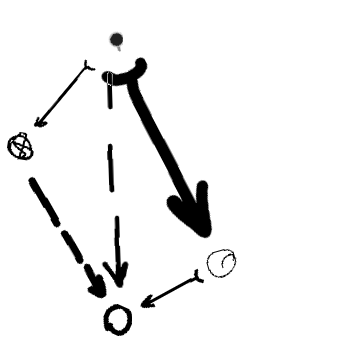
\includegraphics[width=\textwidth]{images/pre_crop.png}
        \caption{}
        \label{fig:pre_crop}
    \end{subfigure}
    \begin{subfigure}[b]{0.3\textwidth}
      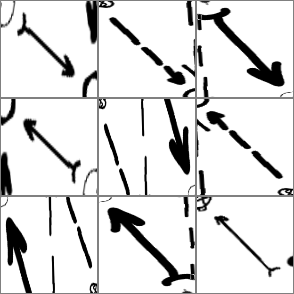
\includegraphics[width=\textwidth]{images/crops.png}
      \caption{}
      \label{fig:crop}
    \end{subfigure}
    \caption{Aus dem links zufällig generiertem Bild wurden die Bilder rechts generiert. Anzumerken ist, dass nur die Bilder der ersten Reihe als korrekt bezeichnet werden.}
    \label{fig:constraint_data}
\end{figure}

Die daraus entstandenen Schnitte (Abbildung \ref{fig:crop}) werden verformt, um einheitliche Ma{\ss}e zu erhalten.
Des Weiteren werden die Bilder so gespiegelt, dass das Anfangsnode stets oben links im Bild ist.
Bilder werden demnach nur als korrekt erkannt, wenn ein enthaltenes Constraint von oben links nach unten rechts dargestellt wird.
Das ist notwendig, um neben der Kategorisierung auch die Richtung der Constraints zu bestimmen.

Aufbauend auf diesen Algorithmen wird eine Datenpipeline programmiert, welche anhand eines Bildes zunächst die Nodes erkennt.
Im nächsten Schritt werden Bildausschnitte generiert, die daraufhin untersucht werden können, ob zwischen zwei Nodes eine Constraint existiert.

Die daraus gewonnene Information kann dann in das von \name{mec2} genutzte JSON-Format überführt und der Mechanismus dargestellt werden.
Damit kann die mechanische Struktur im Sinne einer Bewegungssimulation und Kräfteanalyse weiter verwendet werden.
